% Structure of the dynamodels Model class.
% Build:  pdflatex dynamodels.tex && pdftocairo -svg dynamodels.pdf dynamodels.svg
\documentclass[border=0pt]{standalone}
\usepackage{tikz}
\usepackage{bm}
\usepackage[T1]{fontenc}
\usepackage{helvet}
\renewcommand{\familydefault}{\sfdefault}
\usetikzlibrary{positioning,fit,backgrounds}

% An extra layer below the panel, so the whole figure sits on solid white and
% stays legible on a dark documentation theme.
\pgfdeclarelayer{page}
\pgfsetlayers{page,background,main}

\definecolor{accent}{HTML}{3B6FD4}
\definecolor{ink}{HTML}{16233C}
\definecolor{muted}{HTML}{64748B}
\definecolor{panel}{HTML}{F2F6FC}
\definecolor{edge}{HTML}{C3CFE0}

\begin{document}
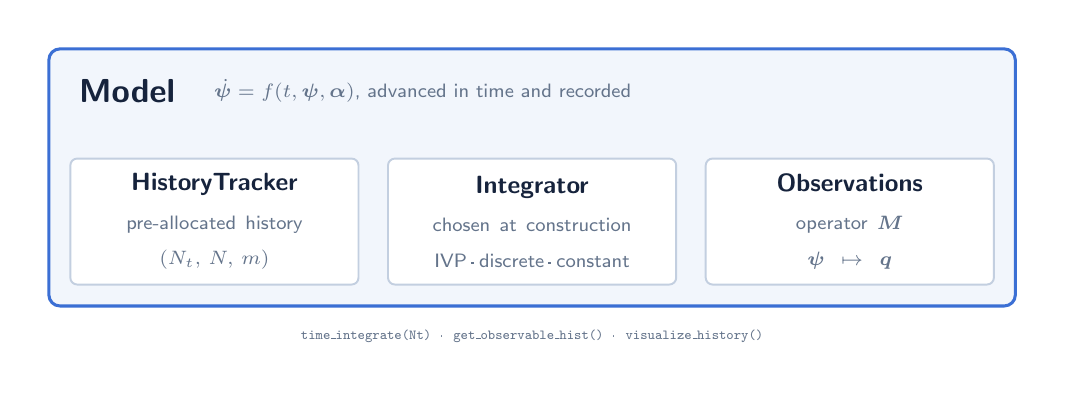
\begin{tikzpicture}[
  box/.style={draw=edge, line width=0.7pt, rounded corners=2.5pt, fill=white,
              text width=33mm, align=center, inner sep=1.8mm, minimum height=16mm},
  hd/.style={text=ink, font=\bfseries\small},
  sb/.style={text=muted, font=\scriptsize}
]

\node[box] (hist) {%
  {\color{ink}\bfseries\small HistoryTracker}\\[0.7mm]
  {\color{muted}\scriptsize pre-allocated history}\\[0.3mm]
  {\color{muted}\scriptsize$(N_t,\, N,\, m)$}};

\node[box, right=3.5mm of hist] (int) {%
  {\color{ink}\bfseries\small Integrator}\\[0.7mm]
  {\color{muted}\scriptsize chosen at construction}\\[0.3mm]
  {\color{muted}\scriptsize IVP\,\textperiodcentered\,discrete\,\textperiodcentered\,constant}};

\node[box, right=3.5mm of int] (obs) {%
  {\color{ink}\bfseries\small Observations}\\[0.7mm]
  {\color{muted}\scriptsize operator $\bm{M}$}\\[0.3mm]
  {\color{muted}\scriptsize$\bm{\psi}\mapsto\bm{q}$}};

\node[anchor=west, hd, font=\bfseries\large] (mtitle) at ([yshift=8.5mm]hist.north west) {Model};
\node[anchor=west, sb] at ([xshift=2.5mm]mtitle.east)
  {$\dot{\bm{\psi}} = f(t,\bm{\psi},\bm{\alpha})$, advanced in time and recorded};

\begin{scope}[on background layer]
  \node[fit=(mtitle)(hist)(int)(obs), draw=accent, line width=1.1pt,
        rounded corners=4pt, fill=panel, inner sep=2.6mm] (model) {};
\end{scope}

\node[below=1.6mm of model, text=muted, font=\ttfamily\tiny] (api)
  {time\_integrate(Nt) \textperiodcentered{} get\_observable\_hist() \textperiodcentered{} visualize\_history()};

\begin{pgfonlayer}{page}
  \fill[white] ([shift={(-2.5mm,-2.5mm)}]current bounding box.south west)
    rectangle ([shift={(2.5mm,2.5mm)}]current bounding box.north east);
\end{pgfonlayer}

\end{tikzpicture}
\end{document}
